\documentclass[../main.tex]{subfiles}

\begin{document}
\section{10.4 - Optimal Control of Pitch/Travel and Elevation with Feedback}
In the previous labs the elevation has been disregarded, and assumed to be zero. In this lab, elevation is not disregarded, and the group had to calculate an optimal trajectory for the elevation as well. The criteria to be minimized was
\begin{equation}\label{eq:lab4_cost_func}
	\phi = \sum_{i=0}^{N-1} (\lambda_{i + 1} - \lambda_f)^{2} + q_1 p_{ci}^2 + q_2 e_{ci} ^2
\end{equation}
and the constraint on the elevation was:
\begin{equation}\label{eq:lab4_elevation_constraint}
	e_k \geq \alpha \text{exp}\left( -\beta (\lambda_k - \lambda_t)^2\right) \forall k \in \left\lbrace 1,...,N\right\rbrace 
\end{equation}

\subsection{The continuous model}
\textit{Answer 10.4.1.1}
The equation for elevation has been given in the problem description as
\begin{equation}\label{eq:lab4_elevation}
	\ddot{e} + K_3K_{ed}\dot{e} + K_3K_{ep}e = K_3K_{ep}e_c
\end{equation}
where $ e_c $ is the elevation setpoint.

Expanding the system defined in \cref{eq:lab2_cont_ss} to include \cref{eq:lab4_elevation}, gives a new system that includes the elevation:

\begin{equation}\label{eq:lab4_cont_ss}
	\underbrace{\begin{bmatrix}
			\dot \lambda \\
			\dot r \\
			\dot p \\
			\ddot p \\
			\dot e \\
			\ddot e \\
	\end{bmatrix}}_{\bm{\dot x}} = 
	\underbrace{
		\begin{bmatrix}
			0 & 1 & 0 & 0 & 0 & 0\\
			0 & 0 & -K_2 & 0 & 0 & 0\\
			0 & 0 & 0 & 1 & 0 & 0\\
			0 & 0 & -K_1 K_{pp} &  -K_1 K_{pd} & 0 & 0\\
			0 & 0 & 0 & 0 & 0 & 1 \\
			0 & 0 & 0 & 0 & -K_3K_{ep} & -K_3K_{ed} \\
		\end{bmatrix}
	}_{\bm A_c}
	\underbrace{
		\begin{bmatrix}
			\lambda \\ r \\ p \\ \dot{p} \\ e \\ \dot{e}
		\end{bmatrix}
	}_{\bm x}
	+
	\underbrace{
		\begin{bmatrix}
			0 & 0 \\
			0 & 0\\
			0 & 0\\
			K_1 K_{pp} & 0\\
			0 & 0 \\
			0 & K_3K_{ep} \\
		\end{bmatrix}
	}_{\bm B_c} 
	\underbrace{
		\begin{bmatrix}
			p_c \\
			e_c \\
		\end{bmatrix}
	}_{\bm u}
\end{equation}

\subsection{The discretized model}
\textit{Answer 10.4.1.2}
Discretizing the continuous system defined in \cref{eq:lab4_cont_ss} was done using the forward Euler method (see \cref{sec:lab2_disc} for more information about this method).

The resulting dicretized system became: 
\begin{equation}\label{eq:lab4_disc_ss}
	\bm A_d = \begin{bmatrix}
		1 & T & 0 & 0 & 0 & 0\\
		0 & 1 & -TK_2 & 0 & 0 & 0\\
		0 & 0 & 1 & T & 0 & 0\\
		0 & 0 & -T K_1 K_{pp} &  1 - T K_1 K_{pd} & 0 & 0\\
		0 & 0 & 0 & 0 & 1 & T \\
		0 & 0 & 0 & 0 & -T K_3 K_{ep} & 1 - TK_3K_{ed} \\
	\end{bmatrix}, \quad
	\bm B_d = \begin{bmatrix}
		0 & 0 \\
		0 & 0\\
		0 & 0\\
		T K_1 K_{pp} & 0\\
		0 & 0 \\
		0 & T K_3K_{ep} \\
	\end{bmatrix}
\end{equation}
where $ T $ is the sample-time.

\subsection{Experimental results}
\textit{Printouts of data from relevant experiments (plots).
Discussion and analysis of the results.
Answer 10.4.2.6 here.}

The group's goal was as in the other labs, to make the helicopter follow the optimal trajectory to $ \lambda_f $ as close as possible. Making the helicopter follow the trajectory consisted of two parts: 
\begin{enumerate}
	\item Tune the LQ regulator to get a good feedback-gain matrix.
	\item Find an optimal trajectory the helicopter could follow.
\end{enumerate}

\subsubsection{Tuning LQ regulator}
Before the group started testing the helicopter's response optimal trajectory found using the SQP-algorithm, the LQ regulator used to find the feedback-gain matrix $\bm K$ had to be tuned. The LQ regulator was exactly the same as the one describe in \cref{kap:task_10_3_LQ_controller}, but now with expanded state and input as described in \cref{eq:lab4_cont_ss}. This means that $ \bm Q $ was now a diagonal matrix of size 6x6, and $ \bm R $ was a diagonal matrix of 2x2. Tuning the LQ regulator is a vital part of achieving as good response. Since the elevation is decoupled from the rest of the states, it should been possible to use the tuning from \cref{sec:lab3_result} and find a good tuning for the elevation (i.e. tuning Q(5,5), Q(6,6) and R(2, 2)). However, in reality the helicopter's state is not decoupled (see \cref{sec:lab4_decoupled}), so to achieve good tuning the group had to tune the whole system again.

A good rule of thumb is that the LQ regulator should be tuned with an input trajectory that one know the helicopter actually can follow. If the helicopter has an input trajectory that is physical impossible to achieve, the tuning will become hard. Therefore, the group tried to create a moderate input-trajectory which seemed reasonable based on their experience from the lab. However, the task was harder than anticipated, and the group did not have enough time to do this. 

Since the group was not able to make a tuning-trajectory for the states and inputs, an optimal trajectory from solving the optimization problem using $q_1 = q_2 = 1$ in the cost function, was used as a replacement. This gave the optimal trajectories shown in \cref{fig:lab4_opt_trajectory}

\begin{figure}[h]
	\centering
	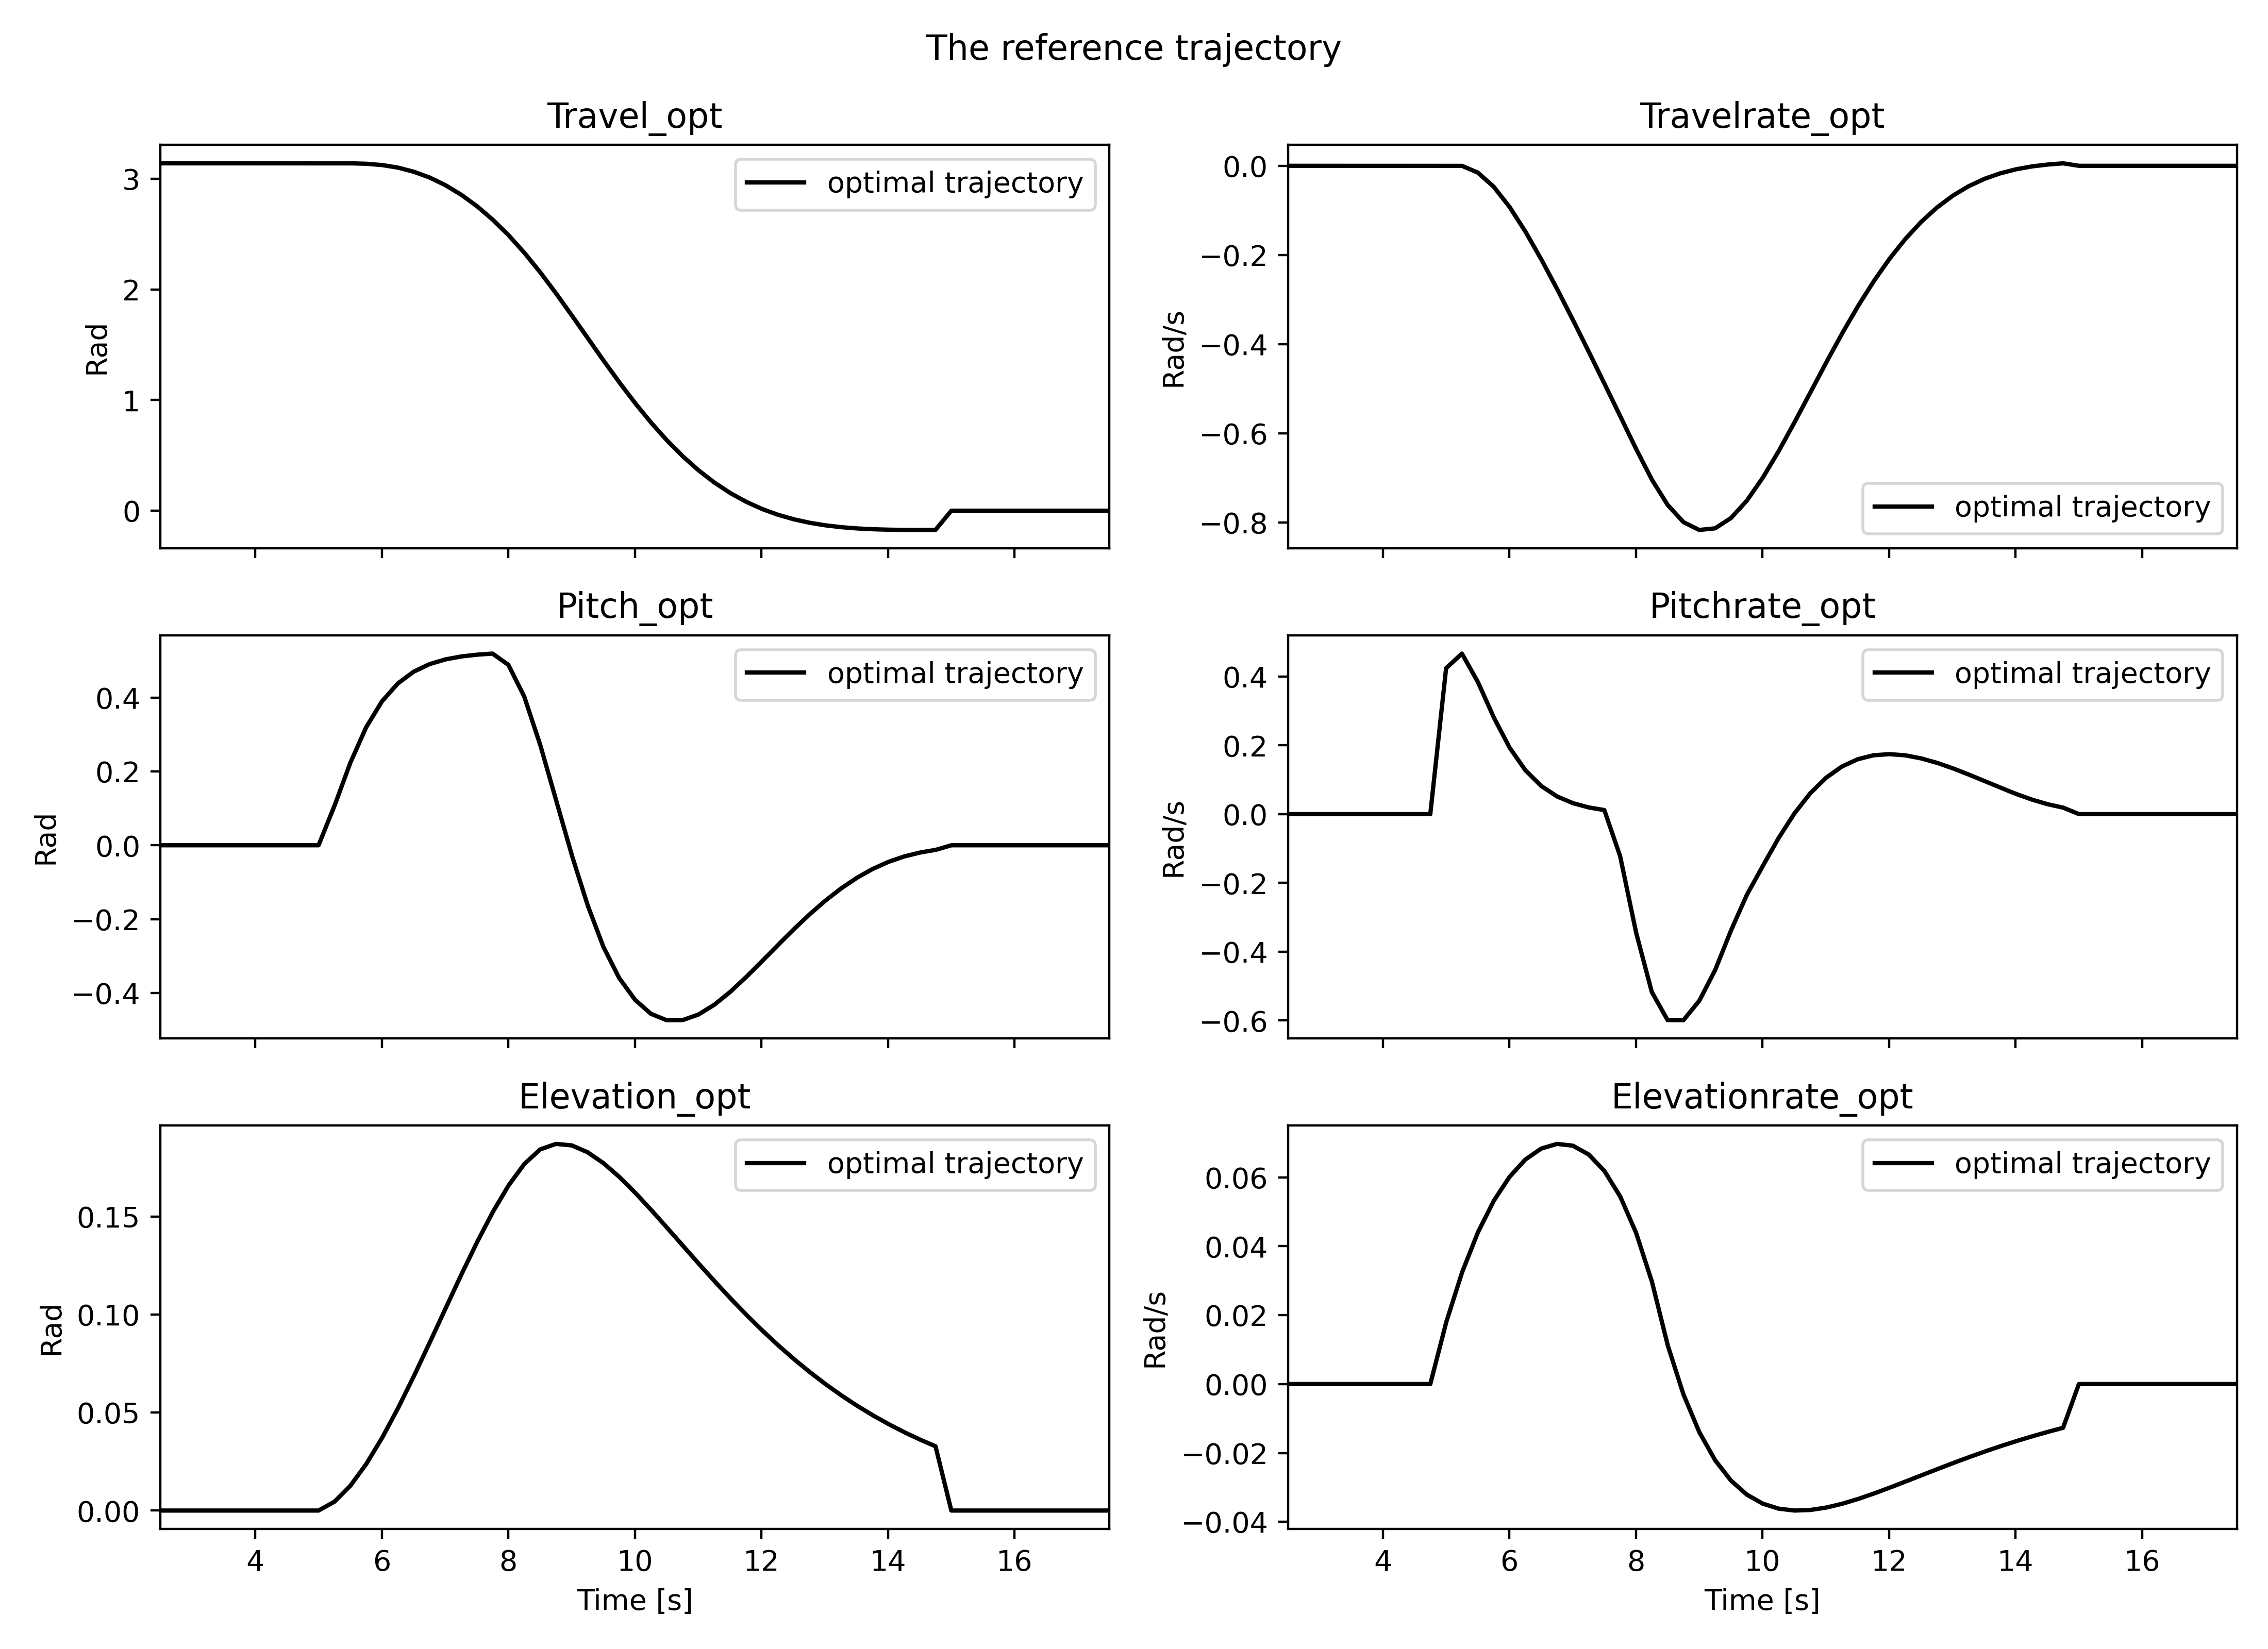
\includegraphics[width=\linewidth]{figures/LAB4_reference_trajectory.png}
	\caption{Optimal trajectories using  $q_1 = q_2 = 1$ in the cost function.}
\end{figure}

In the tuning process we decided to keep $ \bm R $ and $ \bm Q $ as diagonal matrices. $ \bm R $ was set constant equal the identity matrix, i.e. $\bm R = \bm I_2$. The diagonal elements of $ \bm Q $ was then changed to get a good tuning. As in \todo{cref lab3 lqr tuning}each diagonal entry in Q corresponds to the corresponding state in \cref{eq:lab4_cont_ss} \todo{REFORMULATE}. This makes the tuning process simpler since a change in an entry $ \bm Q $ has an expected impact on the response. Higher values of $ \bm Q $ results in inputs with larger magnitude, which again gives a faster response. Having too small values on the diagonal of $ \bm Q $ will therefor give a slow response. Having too large values on the diagonal of $ \bm Q $ will also have unwanted effects as the helicopter approaches a less stable tuning. This is shown in \cref{fig:lab4_diff_Q_values} where the low valued $ \bm Q $ gives a slower response, and a higher valued $ \bm Q $ gives an oscillating response (especially for the pitch rate). The oscillations are noticeable in th ereal world as a shaking helicopter.
\begin{figure}[h]
	\centering
	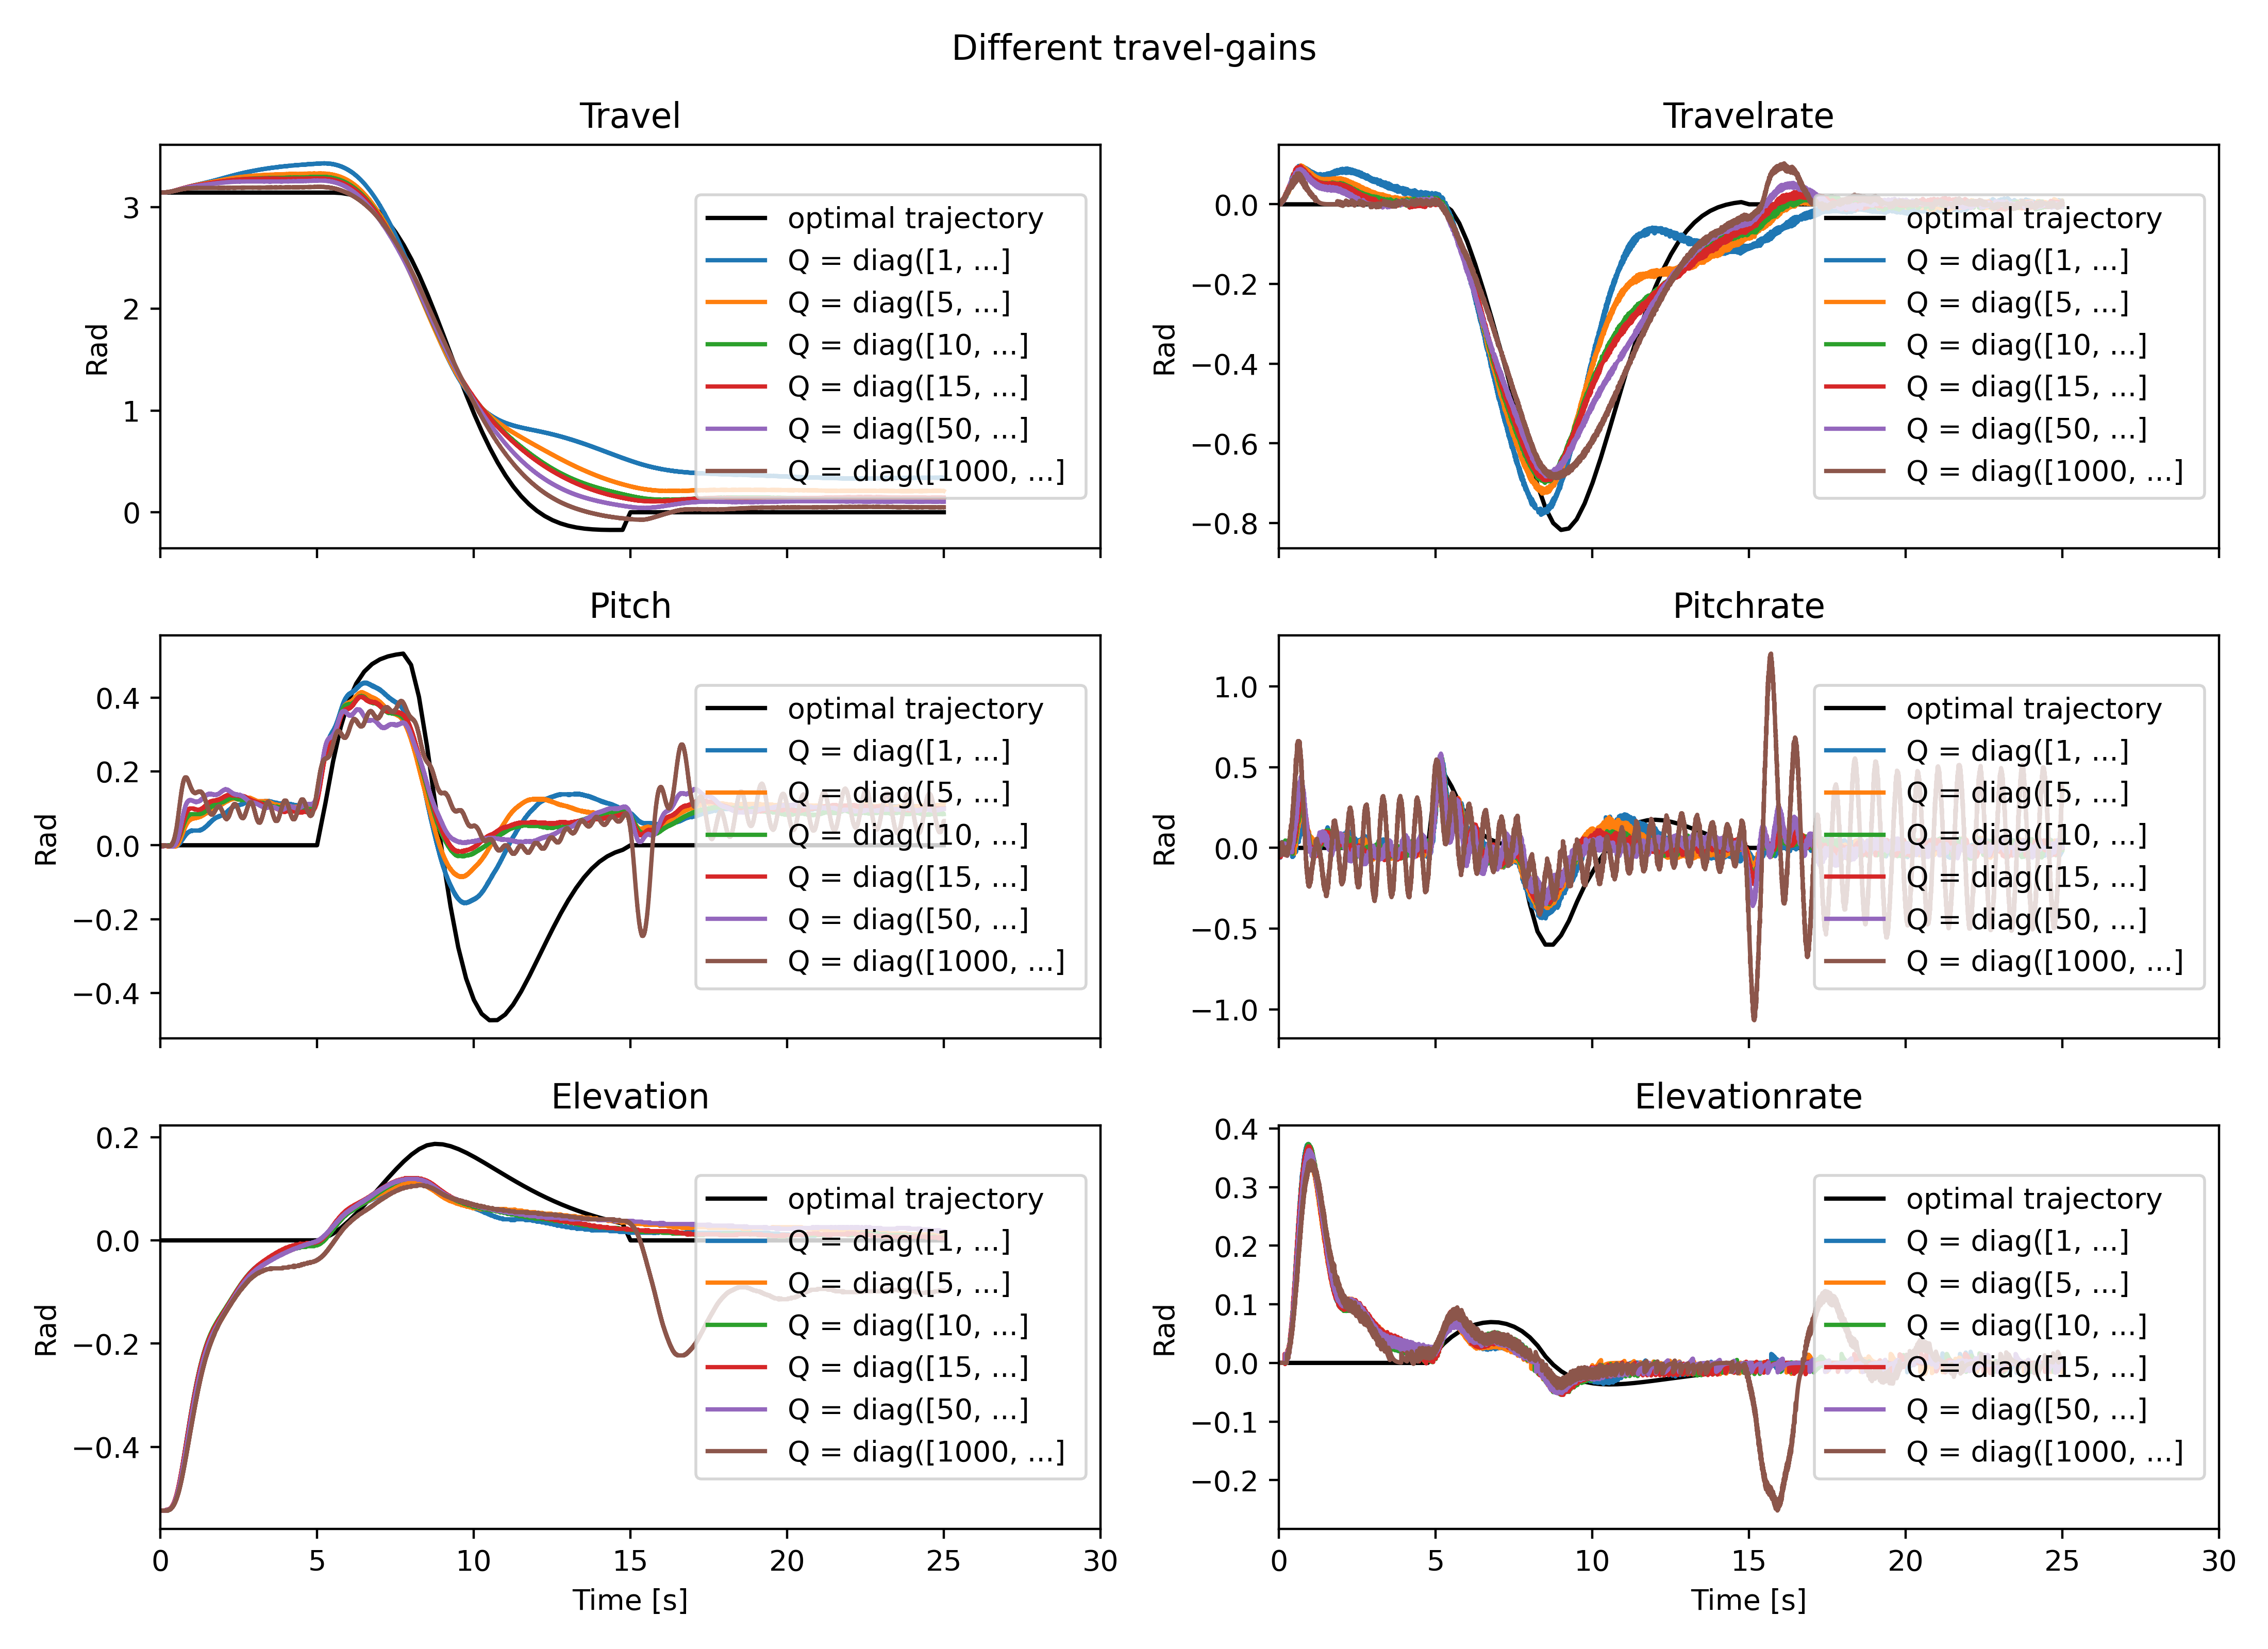
\includegraphics[width=\linewidth]{figures/LAB4_travel_gains.png}
	\caption{Her er alle verdiene vi brukte, bør nok rydde opp litt.}
	\label{fig:lab4_diff_Q_values}
\end{figure}

\begin{figure}[h]
	\centering
	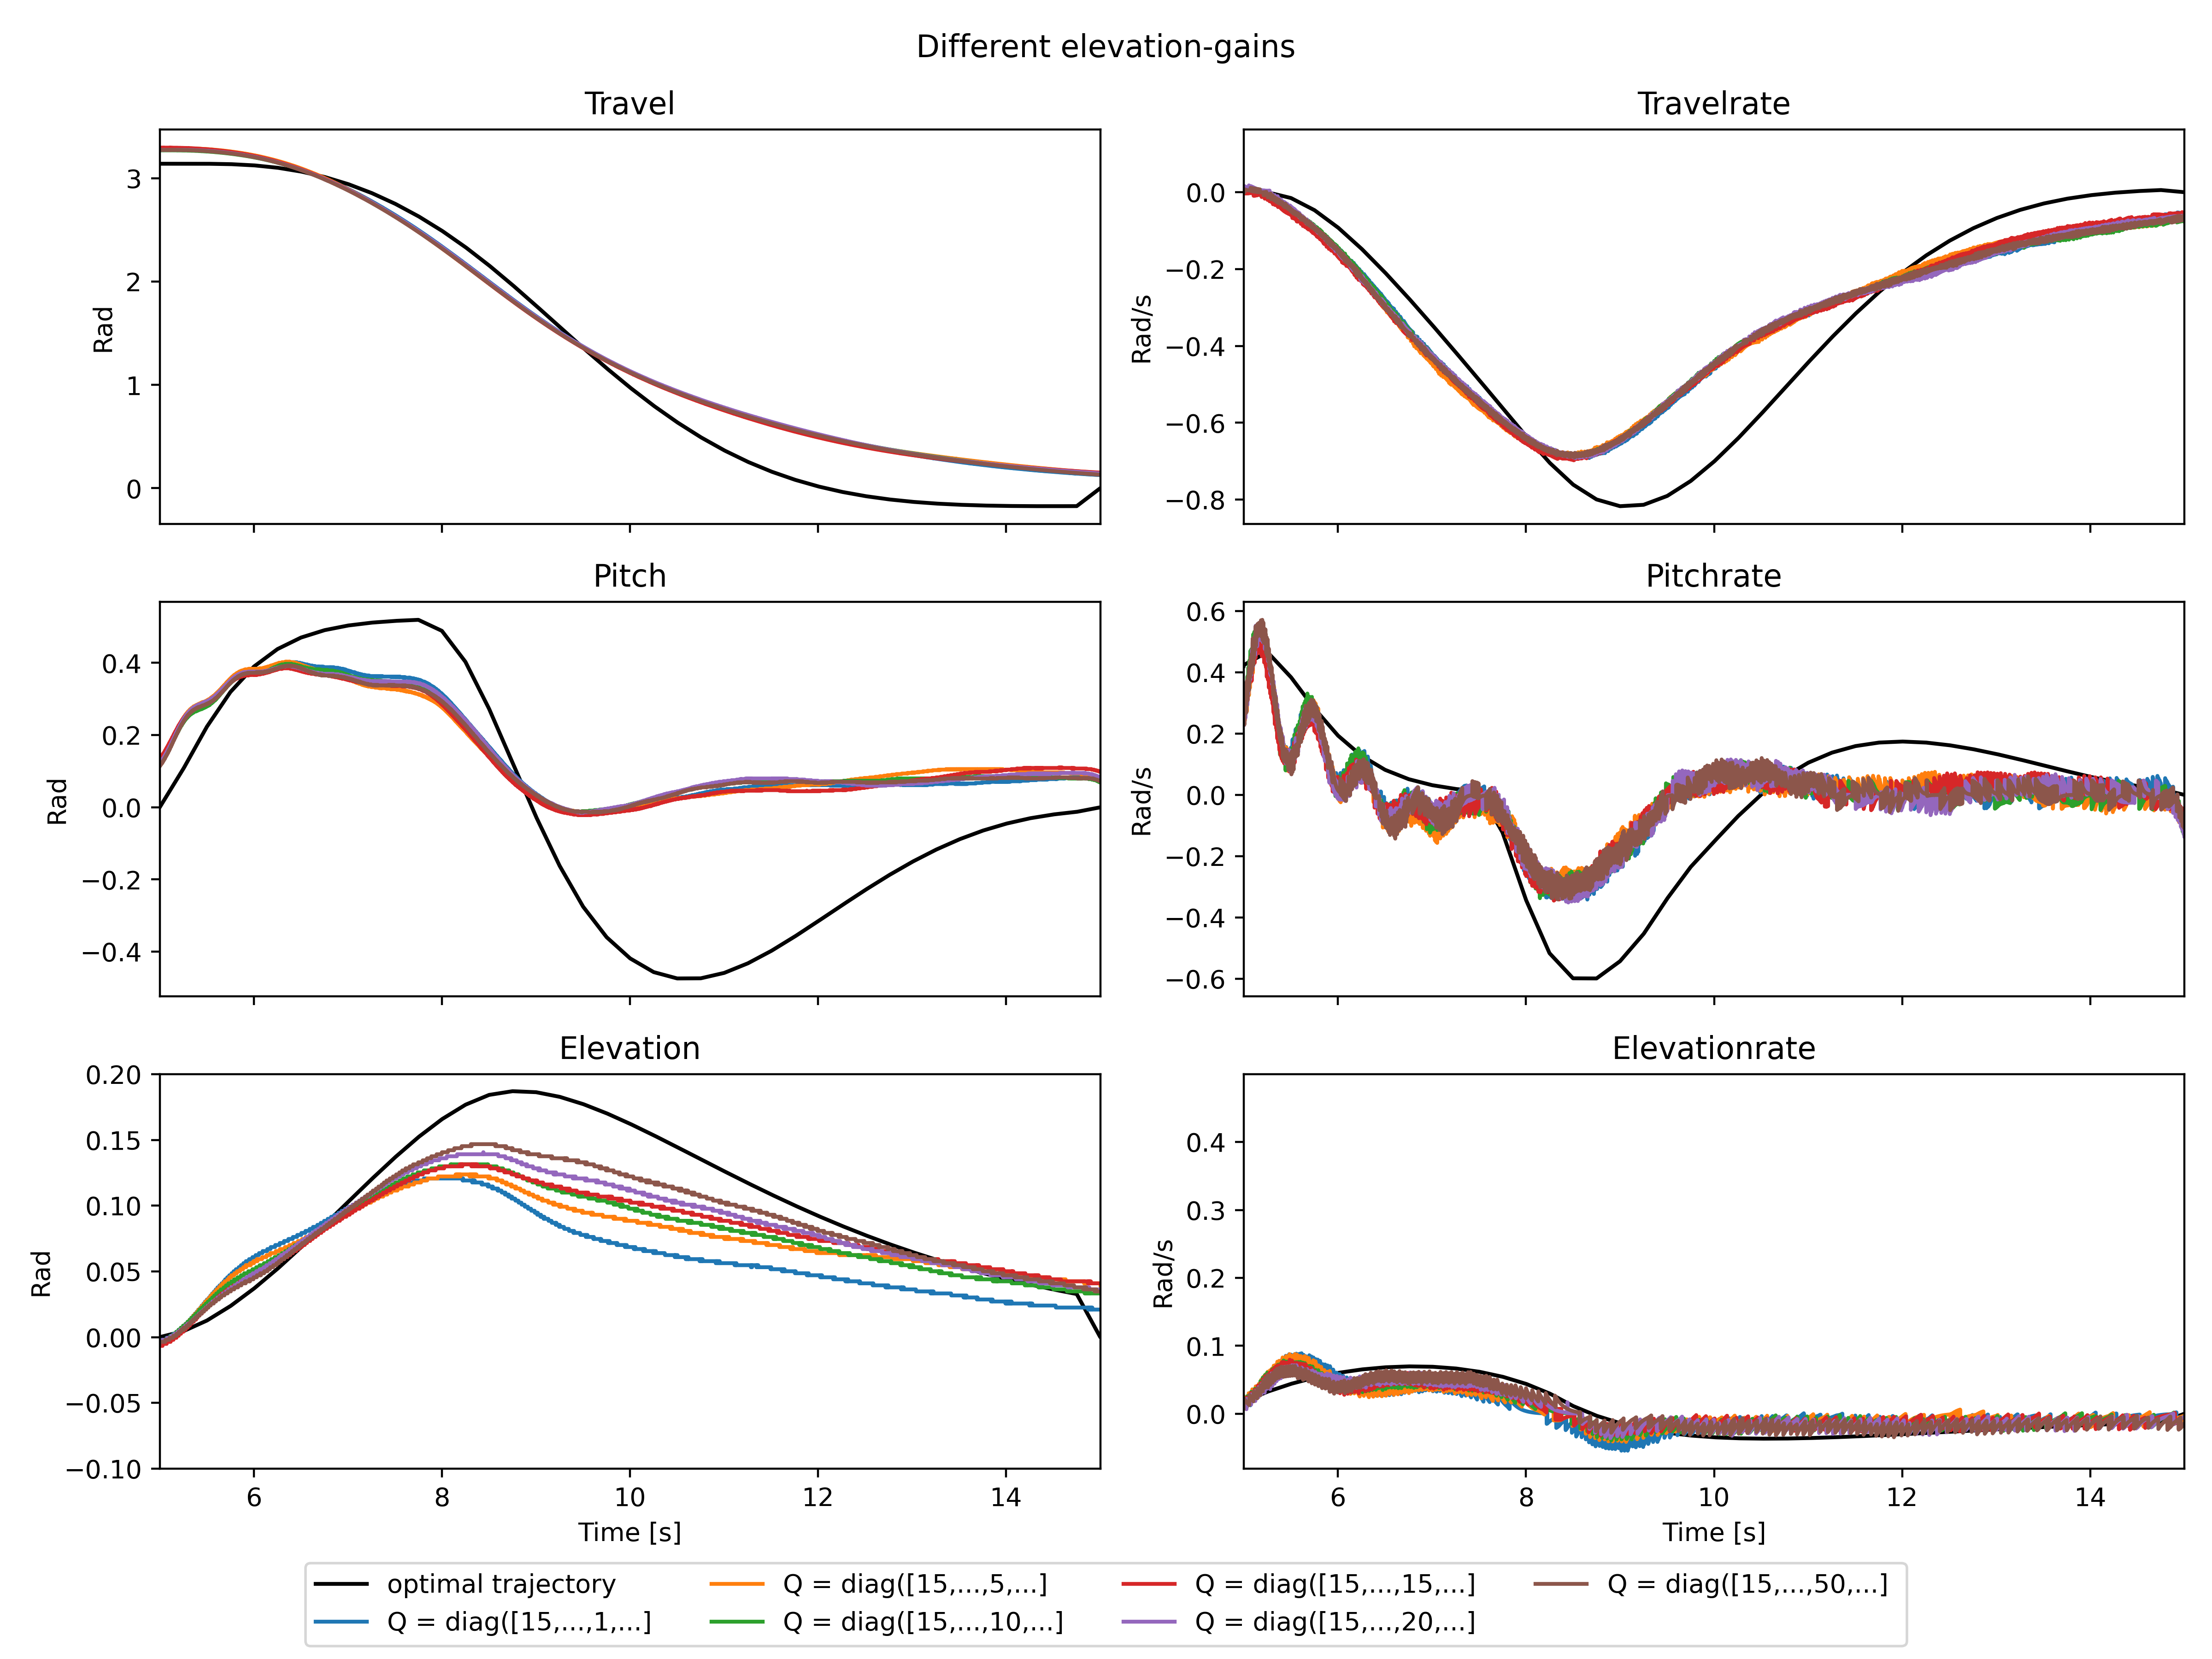
\includegraphics[width=\linewidth]{figures/LAB4_elevation_gains.png}
	\caption{Her er alle verdiene vi brukte, bør nok rydde opp litt.}
	\label{fig:lab4_diff_elevation_values}
\end{figure}

Using the same approach as in \todo{cref lab 3 }the group tuned entry-by-entry in $ \bm Q $. In the end the best tuning was achieved using: 
\begin{equation}\label{key}
	\bm Q = \begin{bmatrix}
		0 & 0 & 0 & 0 & 0 \\
		0 & 0 & 0 & 0 & 0 \\
		0 & 0 & 0 & 0 & 0 \\
		0 & 0 & 0 & 0 & 0 \\
		0 & 0 & 0 & 0 & 0 \\
	\end{bmatrix}, 
	\bm R = \begin{bmatrix}
		1 & 0 \\ 
		0 & 1
	\end{bmatrix}
\end{equation}

This gave the results in \cref{fig:LAB4_best_tuning}
\begin{figure}[h]
	\centering
	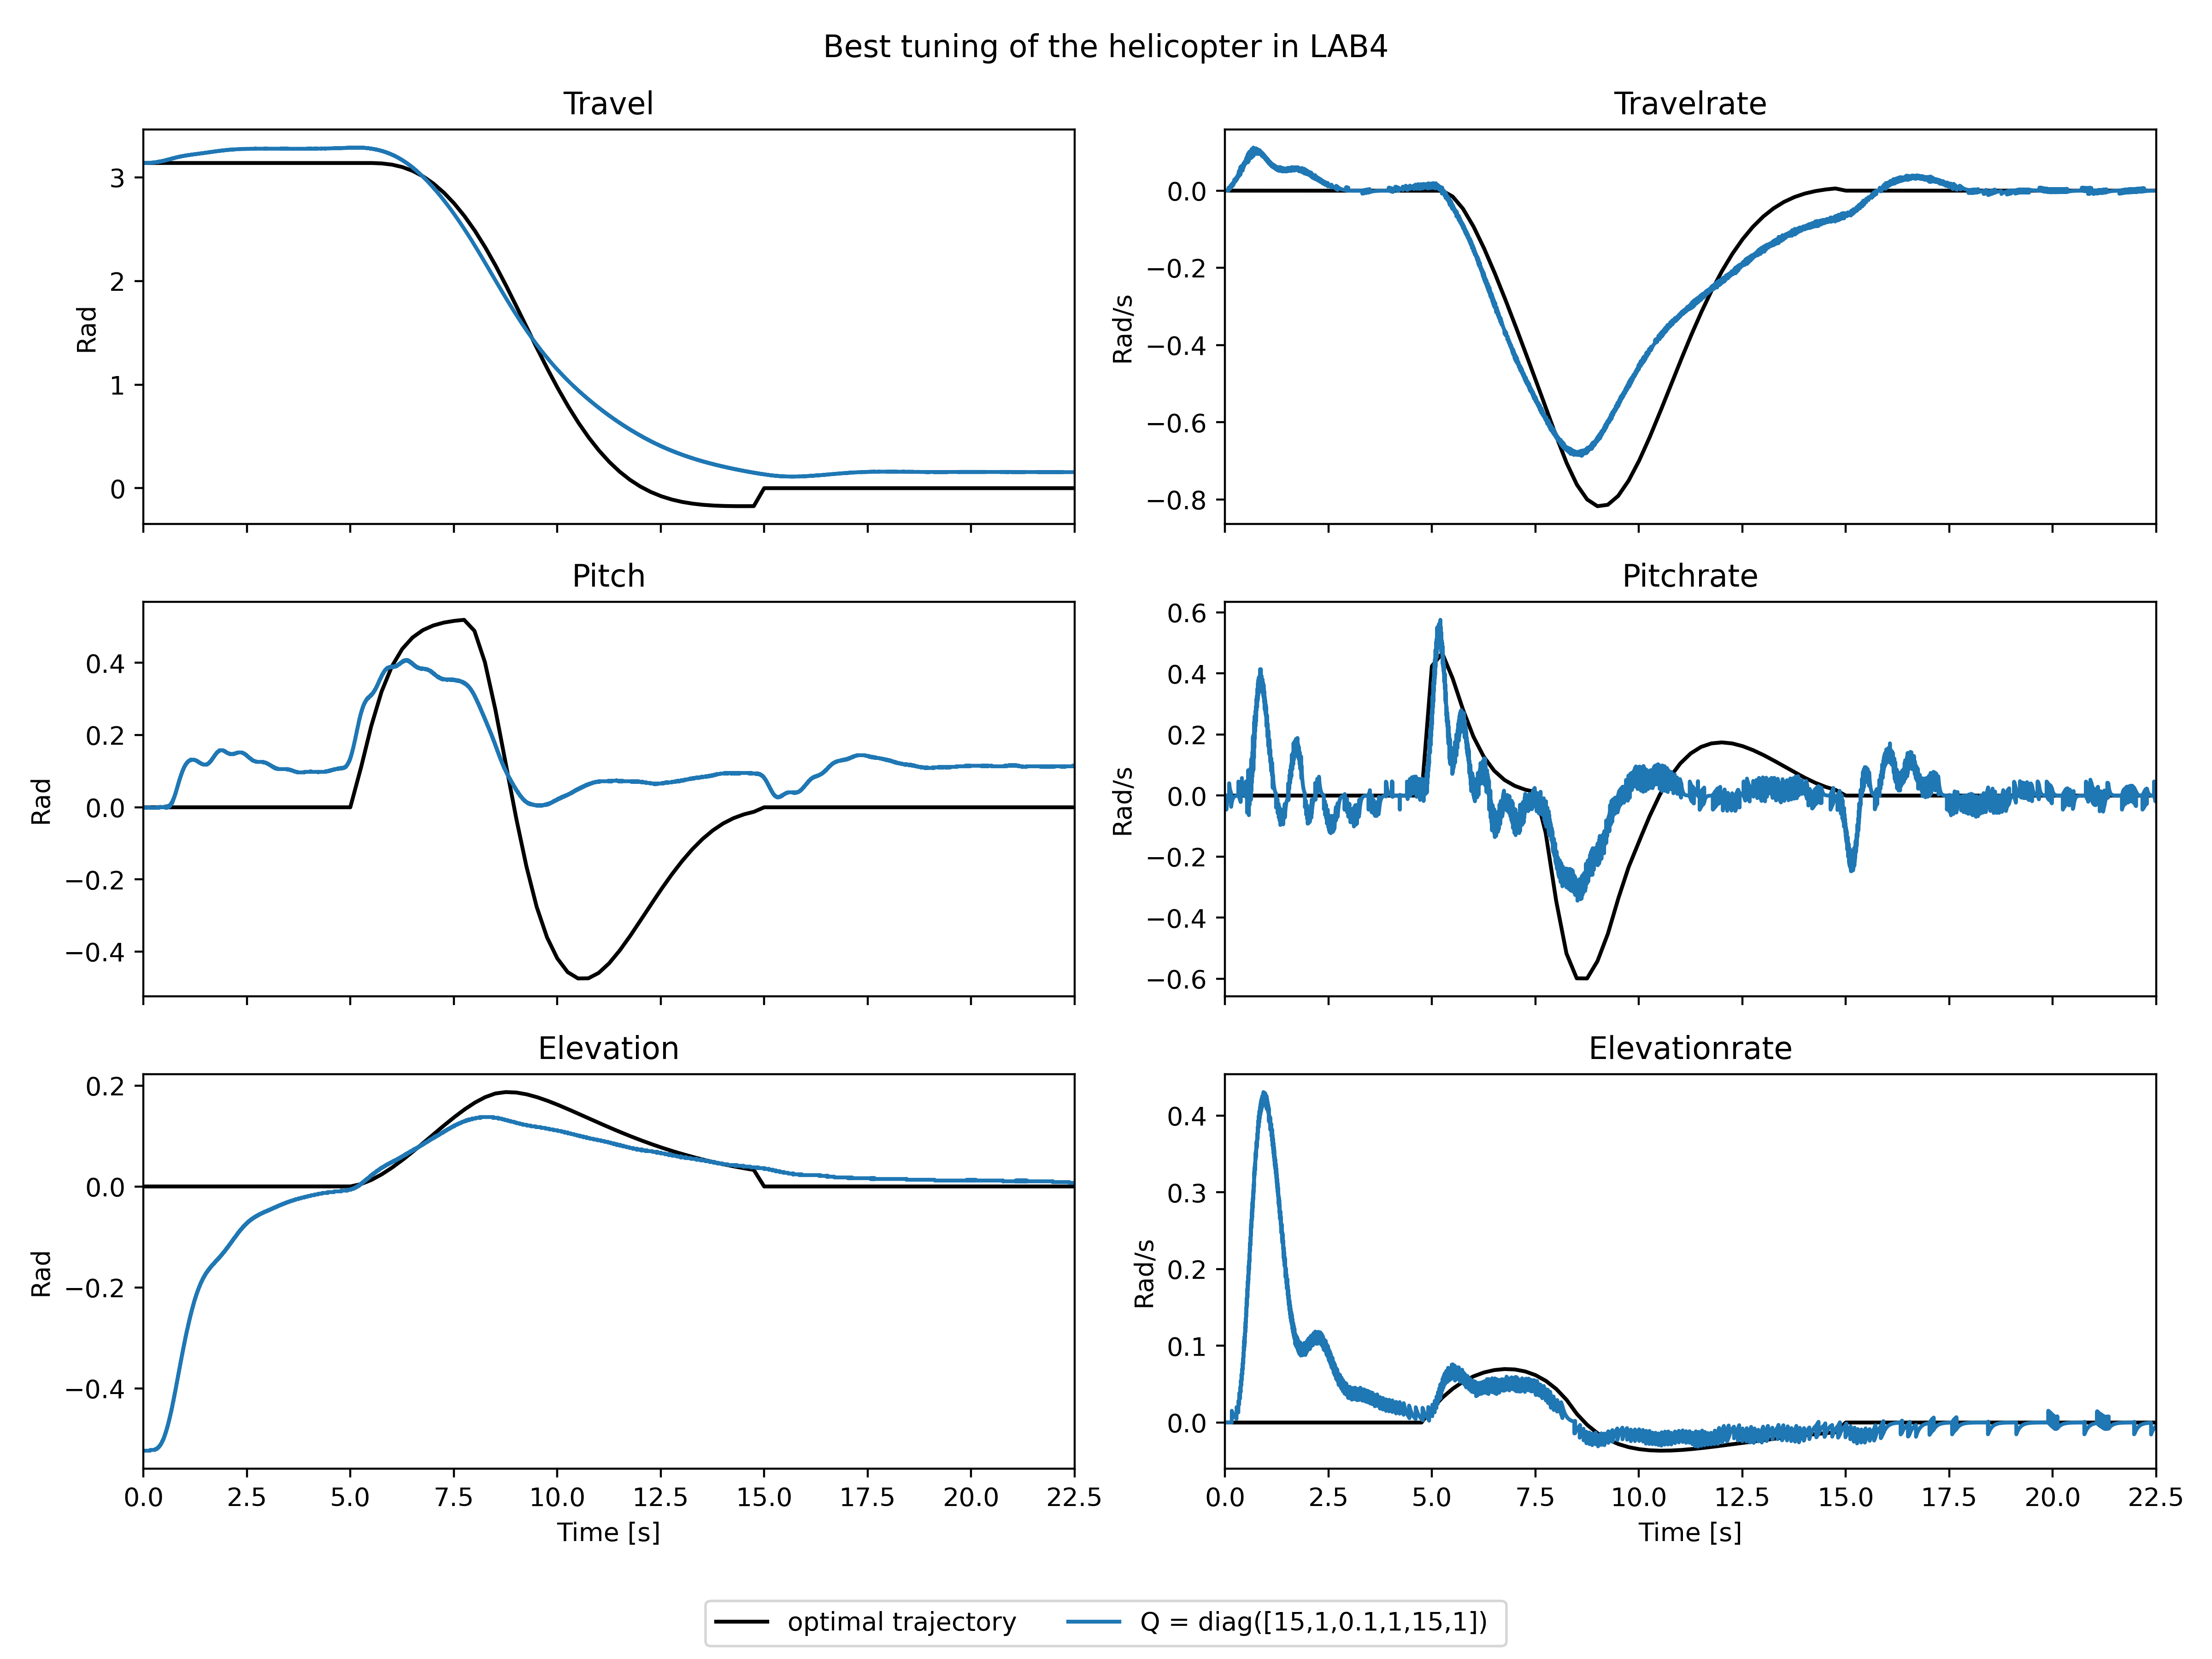
\includegraphics[width=\linewidth]{figures/LAB4_best_tunings.png}
	\caption{Best tuning}
	\label{fig:LAB4_best_tuning}
\end{figure}

\subsubsection{Finding a reasonable trajectory}
With a good
 

\subsection{Decoupled model} \label{sec:lab4_decoupled}
\textit{Answer 10.4.2.7}
As states in the problem description, the two last states are completely decoupled from the first four states. Or put in other words, the dynamics describing elevation is completely independent on the pitch and travel. This is of course not the case in reality, and illustrates how ``simple'' are model of the system actually is!

It becomes quite obvious from the plots \todo{Fin plots that shows this} that the elevation response is heavily coupled with both pitch and travel. Plot \todo{add cref} shows this as when the pitch is changed at time \todo{add time point}, the elevation also changes when it in fact should have been still as calculated in the optimal trajectory. Also there is a lot of rotational forces that have not been considered in the model. E.g. the travel rate $ r $ will create a centripetal force going along the helicopter arm, and point inwards to the origin of the arm. If the helicopter arm is not completely horizontal, this centripetal force will have a component in the direction of the elevation. The main point is that our model is a very simplified version of the real physics of the helicopter. In reality the helicopter is a complex system, which we can never define 100 \% exact with a mathematical formulation. It is impossible.

The effect this has on our optimal trajectory, is that our solver considers elevation as a system that is completely independent on the other states. The implication of this is that our optimal trajectory for elevation is the same, no matter how the trajectory for pitch and travel looks like. \todo[inline]{Is this statement correct? Test this} This can of course be turned the other way around, as the optimal pitch- and travel-trajectory is also independent on the optimal elevation trajectory. The optimal trajectories are ``wrong'', since the elevation is clearly not independent on the other states! Our helicopter will therefor have a hard time following the optimal trajectories as they are not a good representation of the reality.

\subsubsection{Possible solutions}
There are no correct solution to this problem, as we will never be able to describe the real-world system exact with mathematical formulations. There are however, some ``solutions'' that will improve our system and reduce the errors that arises from our decoupled model.

The obvious solution is to couple the model by making it more realistic. There are forces that we can include in our model to make it more accurate. These are for instance the centripetal force mentioned above, friction forces, forces caused by the ground effect, and so on. Of course we can only add simplified equations for these forces, but it would nevertheless increase the accuracy of our model! We will never be able to take into account all forces, and many forces are actually impossible to model mathematically. Therefore we need to identify the forces that has the biggest impact on the error in our model. This is a hard task in itself and can be considered a downside of this approach. Another downside is that our model will quickly become complex and hard to understand. However, the group thinks that it would not be to much work to take into account the most obvious rotational forces, which could possibly cause a big improvement in the optimal solution.

Another solution is not to change the mathematical model of the helicopter at all, but rather change the regulator for the helicopter. Maybe adding integral-effect in the pitch- and elevation-controller would help decreasing the error? Or maybe other feedback-loop implementations could yield better results? There are many possible solutions to improve the regulation of the helicopter! Using this ``solution'', our optimal solution will still be wrong, but we can reduce the error by using a better regulator. The advantage of this is that we can spend less time making a more exact mathematical model, and rather focus on making a regulator that is more robust for errors. The disadvantage is of course that our optimal trajectories are still wrong.



\subsection{MATLAB and Simulink}
\textit{Code and diagrams go here}

\subsection{Optional exercise}
\textit{Which constraints did you add? What was the results? Plots? Discussion?}
\end{document}